\chapter{基于马尔科夫链的分布式聚类算法}

\section{*****************引言}
列出目前分布式轨迹聚类或者说分布式聚类的处理方法,即传输原型向量或概率密度估计的方法。

阐述这样做的缺点,可以添加图。

分布不确定性和高维数据生成模型估计问题

\section{基于马尔科夫链的分布式聚类算法}

\sucsection{总体方案}
为了避免分布不确定性问题和高维数据生成模型轨迹问题,我们提出基于马尔科夫链的分布式聚类算法(MCD-Clustering)。为了避免分布不确定性问题,很自然想到直接传输属地数据概率分布模型参数到中心节点,这种方法在数据量大和数据维度低时使用,而一条具有500个二维坐标点的轨迹数据可以将其看做维度为1000的数据,此时估计数据概率分布模型的方法将不再使用,我们必须通过另外一种模型来估计轨迹数据的概率分布模型。因为每条轨迹各个点之间显然不是独立于彼此的,故当我们将轨迹数据看做是高维数据时,由于每条轨迹数据相邻点存在相关性,可以看做维度和维度之间存在相关性,我们基于这种认知提出使用马尔科夫链来模拟一簇相似轨迹的生成模型,于是提出了基于马尔科夫链的分布式聚类算法(MCD-Clustering)。方案大致流程如图\ref{ch4frame}所示解:
\begin{figure}[h]
	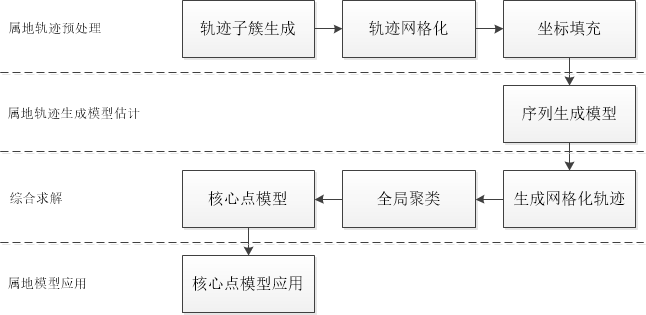
\includegraphics[height=4.5cm,width=7.5cm]{ch4frame.png}
	\caption{MCD-Clustering 算法框架}
	\label{ch4frame}
\end{figure}

整个方案可以分为四个部分:属地轨迹预处理、属地轨迹生成模型估计、综合求解和属地模型应用。属地轨迹预处理,该阶段分为三个步骤:轨迹子簇生成、轨迹数据网格化和轨迹坐标填充。为了通过马尔科夫链能够更好的估计轨迹生成模型,首先对属地轨迹数据集进行聚类操作来得到多个轨迹子簇,我们假设一个子簇里面的轨迹大部分有着相同的轨迹形状。子簇生成后,针对每个子簇中的轨迹进行网格化操作,网格化的作用是通过更少数量的共用坐标点来表示子簇中所有轨迹中的坐标点。由于传感器在采样运动物体轨迹时存在不同物体速度的差异,所以经常会出现一条轨迹时间上相邻的坐标点在网格坐标中并不相邻,此时需要在这两个网格中不相邻的点以指定的策略补充一些坐标点,使得所有轨迹中时间上相邻的点在网格中也相邻。属地轨迹生成模型估计,通过马尔科夫链模型来模拟轨迹生成模型,利用属地轨迹数据集写出含有马尔科夫链参数的最大似然函数,利用最优化理论方法求得使最大似然函数取最大值的马尔科夫链参数。综合求解和属地模型应用,属地将求得的马尔科夫链参数传递给中心节点,中心节点通过这些参数重新生成轨迹坐标,利用重新生成的轨迹坐标作为全局聚类的输入,经过全局聚类输出若干簇心向量,将所有的簇心向量传递给各个计算节点,计算节点利用通过全局聚类计算出的簇心向量来对未知轨迹进行异常检测。

在进入方案具体流程之前,首先对常用符号进行定义。

假设计算节点的轨迹数据集记为D,轨迹数据集包含有n条轨迹,每条轨迹由m个坐标点构成,坐标点的维度为2,即:
\[
D=\left\{ t_1,t_2,...,t_n \right\} 
\\
t=\left\{ \left( x_1,y_1 \right) ,\left( x_2,y_2 \right) ,...,\left( x_m,y_m \right) \right\} 
\]

轨迹数据通过聚类算法产生的簇集合记为$C=\left\{ C_1,C_2,...,C_k \right\} $,其对应的簇心向量记为$\mu =\left\{ \mu _1,\mu _2,...,\mu _k \right\} $。


\subsection{属地轨迹预处理}

属地轨迹预处理分为三个阶段:轨迹子簇生成、轨迹数据网格化和轨迹坐标填充。

轨迹子簇生成阶段主要通过聚类算法来实现,本节选择k-means++算法进行聚类,通过聚类算法生成的轨迹子簇记为集合C,其中聚类中使用的距离度量与第三章定义的距离一样,假设两条轨迹a和b,则轨迹a和b之间的距离为:
\[
\text{Dist}\left( \text{a},\text{b} \right) =\frac{1}{m}\sum_{i=1}^m{\sqrt{\left( a_{x}^{i}-b_{x}^{i} \right) ^2+\left( a_{y}^{i}-b_{y}^{i} \right) ^2}}
\]

k-means++聚类在选择k值时需要聚类评价指标来评判不同k值下的聚类效果,这里采用内部指标DI来衡量,DI表达式如式\ref{DI}所示。
k-means++初始化操作如下:\\
\begin{algorithm}[H]
	 \KwData{样本集$D=\left\{t_1,t_2,...,t_n\}\right\}$,簇个数K}
	 \KwResult{簇心向量$\mu=\left\{\mu_1,\mu_2,...,\mu_K\}\right\}$}
	 从数据集D中随机初始化1个样本,将其作为第一个簇的簇心$\mu={\mu_1}$\;
	 \Repeat{k=2,3,...,K}{
	 	R=D-$\mu$
	 	\For{$t_i$ in R}{
	 		计算$P(x_i)$,$P\left( t_i \right) =\omega \sum_{\mu _i\in \mu}{\left( t_i-\mu _i \right) ^2}$,其中$\omega$是归一化系数\;\\
	 	}
	 	按照R集合中所有点的概率分布选出$\mu_k$,将其加入集合$\mu$\;\\
	 }
	 \caption{kmeanspp_initialization}
\end{algorithm}

轨迹子簇生成的具体流程如下:\\
\begin{algorithm}[H]
	\label{kmeanspp}
	 \KwData{样本集$D=\left\{t_1,t_2,...,t_n\}\right\}$,簇个数K,阈值S}
	 \KwResult{簇划分$C=\left\{C_1,C_2,...,C_K\}\right\}$,簇心向量$\mu=\left\{\mu_1,\mu_2,...,\mu_K\}\right\}$}
	 K=2\;\\
	 kmeanspp_initialization\(D,K\)\;
	 C,$\mu$=kmeans\(D,K\)\;
	 $DI_K$=DI(C)\;
	 flag=true\;
	 \Repeat{flag}{
	 	K=K+1\;
	 	kmeans_initialization\(D,K\)\;
	 	C,$\mu$=kmeans\(D,K\)\;	
	 	DI_K=DI(C)\; 
	 	\If{$DI_K-DI_{K-1}\leqslant S$}{
	 		flag=false\;
	 	}	
	 }
	 \caption{轨迹子簇生成流程}
\end{algorithm}

轨迹子簇生成后,针对每个子簇进行网格化。原始轨迹数据中的坐标点在二维连续空间上取值,将轨迹数据网格化后,轨迹所有坐标点在二维离散网格空间取值。最简单的网格化则是将二维连续空间中的点坐标取整,即将二维连续空间映射到由所有整数构成的坐标形成的二维离散网格空间,如图\ref{gridization}所示。
\begin{figure}[h]
	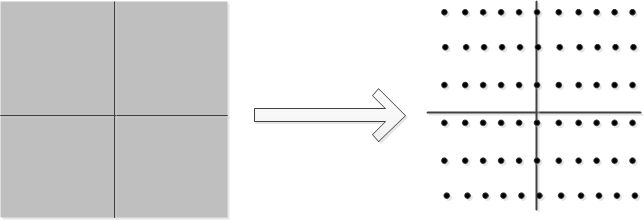
\includegraphics[height=4.5cm,width=7.5cm]{gridization.png}
	\caption{空间网格化}
	\label{gridization}
\end{figure}

对于轨迹数据可以采用同样的方法对其进行网格化,网格化规则可以通过下面式子表示:
\begin{center}
f\left( x \right) =\left\{ \begin{array}{c}
	sign\left( x \right) *\left( \lfloor x \rfloor +1 \right) \,\,if\,\,|x-\lfloor x \rfloor |>0.5\\
	sign\left( x \right) *\left( \lfloor x \rfloor -1 \right) \,\,if\,\,|x-\lfloor x \rfloor |\leqslant 0.5|\\
\end{array} \right\\
\varPhi \left( \left( x,y \right) \right) =\left( f\left( x \right) ,f\left( y \right) \right)\\
g\left\{ \left( x_1,y_1 \right) ,\left( x_2,y_2 \right) ,...,\left( x_l,y_l \right) \right\} =\left( x_1,y_1 \right) \,\, if\,\,\left( x_1,y_1 \right) =\left( x_2,y_2 \right) =...=\left( x_l,y_l \right)
\end{center}


其中,sign(x)表示实数x的符号。通过上式规则对轨迹中的每一个坐标点进行网格化,图\ref{gridization}展现了轨迹经过网格化后的效果,图\ref{originaltrajectory}表示原始轨迹数据,图\ref{gridedtrajectory}表示网格化后的轨迹数据。网格化对轨迹数据的精度造成了一定程度的影响,但是完全不影响其对轨迹形状的刻画。
\begin{figure}[h]
\subfigure[]{
\label{originaltrajectory}
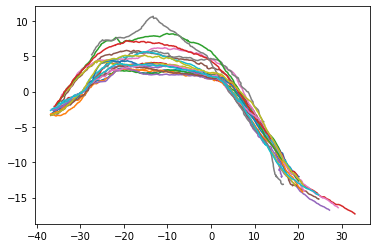
\includegraphics[width=6.77cm]{originaltrajectory.png}}
\subfigure[]{
\label{gridedtrajectory}
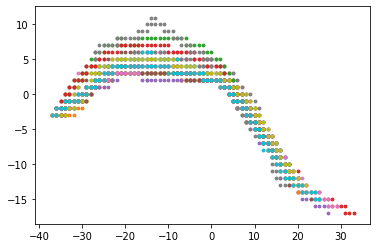
\includegraphics[width=7.04cm]{gridedtrajectory.png}}
\caption{轨迹网格化前后对比}
\label{gridization}
\end{figure}
由于传感器在采样运动物体轨迹时存在不同物体速度的差异,所以经常会出现一条轨迹时间上相邻的坐标点在网格空间中并不相邻,此时需要在这两个网格中不相邻的点之间通过指定的操作填充一些坐标点,使得所有轨迹中时间上相邻的点在网格空间中也相邻,这种保证了网格空间数据相邻性的操作称之为轨迹数据填充操作。假设一条网格化后的轨迹数据记为$g=\left\{ \left( x_1,y_1 \right) ,\left( x_2,y_2 \right) ,...,\left( x_l,y_l \right) \right\} $,轨迹数据填充操作流程如下:\\
\begin{algorithm}[H]
 	\KwData{一条网格化的轨迹$g=\left\{ \left( x_1,y_1 \right) ,\left( x_2,y_2 \right) ,...,\left( x_l,y_l \right) \right\} $}
 	\KwResult{轨迹数据填充后的轨迹数据$\hat{g}=\left\{ \left( x_1,y_1 \right) ,\left( x_2,y_2 \right) ,...,\left( x_s,y_s \right) \right\} $}

	 \Repeat{i=1,2,...,l-1}{
	 	\If{$x_i==x_{i+1}$ && $|y_i-y_{i+1}|>1$}{
	 		s = sign($y_{i+1}-y_{i}$)
	 		在坐标$(x_i,y_i)$后面填充坐标$(x_i,y_i+s),(x_i,y_i+2*s),...,(x_i,y_{i+1}-s)$
	 	}
	 	\ElseIf{$y_i==y_{i+1}$ && $|x_i-x_{i+1}|>1$}{
	 		s = sign($x_{i+1}-x_i$)
	 		在坐标$(x_i,y_i)$后面填充坐标$(x_i+s,y_i),(x_i+2*s,y_i),...,(x_{i+1}-s,y_{i})$
	 	} 
	 	\ElseIf{$|x_i-x_{i+1}| \geqslant 1$ && $|y_i-y_{i+1}| \geqslant 1$}{
	 		xs = sign($x_{i+1}-x_i$)
	 		ys = sign($y_{i+1}-y_{i}$)
	 		在坐标$(x_i,y_i)$后面填充坐标$(x_i+xs,y_i),(x_i+xs,y_i+ys)$
	 		\While{假设最后填充的坐标$(x_t,y_t)$不满足:$x_t==x_{i+1}$ || $y_t==y_{i+1}$ || ($|x_t-x_{i+1}|==1$ && $|y_t-y_{i+1}|==1$) }{
	 			在坐标$(x_t,y_t)$后面填充坐标$(x_t+xs,y_t),(x_t+xs,y_t+ys)$
	 		}
	 		\If{$x_t==x_{i+1}$ && $|y_t-y_{i+1}|>1$}{
	 			s = sign($y_{i+1}-y_{t}$)
	 			在坐标$(x_t,y_t)$后面填充坐标$(x_t,y_t+s),(x_t,y_t+2*s),...,(x_t,y_{i+1}-s)$
	 		}
	 		\ElseIf{$y_t==y_{i+1}$ && $|x_t-x_{i+1}|>1$}{
	 			s = sign($x_{i+1}-x_t$)
	 			在坐标$(x_t,y_t)$后面填充坐标$(x_t+s,y_t),(x_t+2*s,y_t),...,(x_{i+1}-s,y_{t})$
	 		}
	 		\ElseIf{$|x_t-x_{i+1}|==1$ && $|y_t-y_{i+1}|==1$}{
	 			s = sign($x_{i+1}-x_t$)
	 			在坐标$(x_t,y_t)$后面填充坐标$(x_t+s,y_t)$
	 		}
	 	}
	 }
	 \caption{轨迹数据填充操作}
\end{algorithm}

\subsection{属地轨迹生成模型估计}
针对轨迹数据网格化和轨迹数据填充后的轨迹子簇,通过马尔科夫链模型来估计其轨迹生成模型。假设子簇C中含有l条轨迹$C=\left\{ t_1,t_2,...,t_l \right\} $,因为每条轨迹都需要经过轨迹数据网格化和轨迹数据填充两个操作,故子簇C中每条轨迹包含的坐标点个数将不再相同。记子簇中轨迹所有坐标点的集合为S,集合S中元素个数为|S|,将集合S中的每一个元素看做是马尔科夫链中的一种状态,其转移矩阵记为P可表示为:
\begin{equation}
\label{transitionmatrix}
P=\begin{matrix}{c|cccc}
	&		s_1&		s_2&		\dots&		s_{|s|}\\
	\hline
	s_1&		p_{11}&		p_{12}&		\dots&		p_{1|s|}\\
	s_2&		p_{21}&		p_{22}&		\dots&		p_{2|s|}\\
	\vdots&		\vdots&		\vdots&		\ddots&		\vdots\\
	s_{|s|}&		p_{|s|1}&		p_{|s|2}&		\cdots&		p_{|s||s|}\\
\end{matrix}
\end{equation}

轨迹子簇C对应的似然函数可以表示为:
\[
L=p_{11}^{n_{11}}*p_{12}^{n_{12}}*p_{1|s|}^{n_{1|s|}}*...*p_{|s||s|}^{n_{|s||s|}}
\]

对上式对数似然函数取对数不影响似然函数取最大值时的参数取值,故轨迹子簇C对应的对数似然函数可以表示为:
\begin{equation}
\label{ch4ll}
LL=n_{11}\ln \left( p_{11} \right) +n_{12}\ln \left( p_{12} \right) +...+n_{|s||s|}\ln \left( p_{|s||s|} \right) 
\end{equation}
求解式\ref{ch4ll}的最大值所得参数矩阵作为马尔科夫链转移矩阵。

为了更清楚上式的求解过程,我们针对其中任意一个状态A的转移概率来进行求解,假设状态A在轨迹子簇C中可以转移到状态B、状态C和状态D,对应的转移概率记为$p_1,p_2和p_3$,且在轨迹子簇C中发生的次数分别记为$n_1,n_2和n_3$,设定轨迹子簇C包含的轨迹数据是充分的,即状态A只能转移到以上三个状态,此时则有:$p_1+p_2+p_3=1$。针对状态A的对数似然函数可以表示为:
\[
LL\left( A \right) =n_1\ln \left( p_1 \right) +n_2\ln \left( p_2 \right) +n3\ln \left( 1-p_1-p_2 \right) 
\]

LL(A)分别对$p_1$和$p_2$求导:
\[
\begin{cases}
	\frac{\partial LL\left( A \right)}{\partial p_1}=\frac{n_1}{p_1}+\frac{-n_3}{1-p_1-p_2}\\
	\begin{array}{c}
	\frac{\partial LL\left( A \right)}{\partial p_2}=\frac{n_2}{p_2}+\frac{-n_3}{1-p_1-p_2}\\
	p_1+p_2+p_3=1\\
\end{array}\\
\end{cases}
\]

通过求解上式方程组可得到方程组的解为:
\[
\begin{cases}
\begin{array}{c}
	\begin{array}{c}
	p_1=\frac{n_1}{n_1+n_2+n_3}\\
	p_2=\frac{n_2}{n_1+n_2+n_3}\\
\end{array}\\
	p_3=\frac{n_3}{n_1+n_2+n_3}\\
\end{array}    
\end{cases}
\]

依照上式解的形式,转移矩阵可以在O(n)时间复杂度内可以得到。

以上构建的模型在轨迹无交叉点的时候能够使用,当轨迹子簇中大部分轨迹形状走势存在交叉点时,我们可以简单分析这种情形下上式模型的不足之处。假设现有轨迹子簇C如图\ref{cross}所示,轨迹依据时间顺序从左下角依次经过A点和B点,最后经过C点到达整个轨迹的右上角,此时轨迹子簇中许多轨迹存在交叉点A,轨迹在A点既可以转移到B点,同样可以转移到C点,而这两种转移将对应两种完全不同的轨迹走势。当轨迹在A点转移到B点时,依据转移矩阵生成轨迹坐标点时会再次经过A点,然后经过C点,此时轨迹形状走势满足整个轨迹子簇形状走势,如图\ref{A2B};而当轨迹在A点转移到B时,依据转移概率矩阵,轨迹将直接经过C点顺势而上到达轨迹右上角,最终将生成许多类似如图\ref{A2C}的轨迹,而这些轨迹与整个轨迹子簇的轨迹形状走势存在较大的差异。
\begin{figure}[h]
\subfigure[]{
\label{cross}
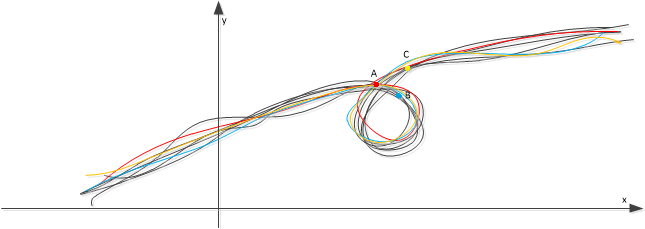
\includegraphics[height=4.5cm,width=4.5cm]{cross.png}}
\subfigure[]{
\label{A2B}
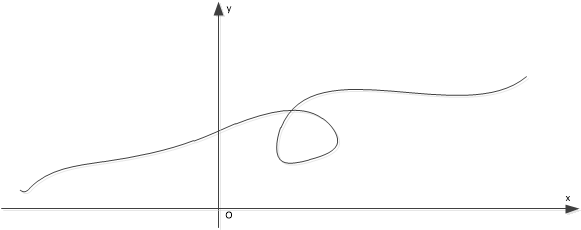
\includegraphics[height=4.5cm,width=4.5cm]{A2B.png}}
\subfigure[]{
\label{A2C}
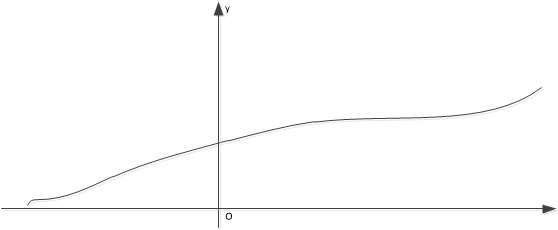
\includegraphics[height=4.5cm,width=4.5cm]{A2C.png}}
\caption{轨迹子簇中存在交叉点的情形}
\label{crosssituation}
\end{figure}

为了解决轨迹子簇中轨迹存在交叉点情况,我们可以将二维的轨迹想象成三维轨迹在平面上的投影,在二维平面上A点是一个点,但对应到三维空间则是两不同个点,只是它们在平面上的投影相同而已。故我们可以将A点对应的状态分成两个状态,记为A1和A2,若轨迹子簇中存在如图\ref{A2C}的轨迹,则这些轨迹经过A点时状态记为A1,过若轨迹子簇中存在如图\ref{A2B}的轨迹,则这些轨迹在经过A点时状态记为A2,将交叉点对应的状态一分为二,后续求解问题则如同轨迹无交叉点的情形一致。通过把交叉点对应状态一分为二的策略,即可在轨迹子簇中轨迹存在交叉点情况下也能准确描述轨迹生成模型。

针对指定的轨迹子簇,其马尔科夫链模型的转移矩阵可以表示为式\ref{transitionmatrix},其状态与轨迹子簇中轨迹坐标点对应,若将马尔科夫链通过图模型表示:所有状态构成图中的点集,状态与状态之间的所有转移构成了图的边集。显然,用于估计轨迹生成模型的马尔科夫链模型对应的图模型不是一个完全图,而是一个稀疏图,因为任意一个状态只能向其在网格空间中相邻的网格点对应的状态进行转移,即任意一个状态只能向极其有限的状态进行转移,这使得马尔科夫链的转移矩阵中存在大量的零元素。于是我们可以通过矩阵稀疏表示方法来代替转移概率矩阵,从而可以减少一部分带宽传输的压力。\\

稀疏矩阵表示方法有很多种,本文采用*****************稀疏矩阵表示


\subsection{综合求解和属地模型应用}
各个计算节点将所有轨迹子簇对应的转移概率矩阵、状态初始分布和轨迹输传输给中心节点,中心节点接收到计算节点传递来的各种参数后,首先将转移概率矩阵稀疏表示还原出原始的轨迹转移矩阵,中心节点通过转移概率矩阵来生成轨迹。假设我们将还原的转移概率矩阵记为A,状态初始概率分布记为$\pi$,轨迹子簇包含的轨迹数量记为N,生成轨迹过程主要流程如下:\\
\begin{algorithm}[H]
	 \KwData{转移概率矩阵A,状态初始概率分布$\pi$,轨迹数量N}
	 \KwResult{生成轨迹集合G}
	 \For{i=1,2,,...,N}{
	 	按照状态初始状态分布$\pi$产生状态$s_1$\;\\
	 	状态$\s_1$在转移概率矩阵中对应的概率分布记为S\;\\
	 	轨迹序列L\;\\
	 	\Repeat{若概率分布S中存在非零元素}{
	 		依据概率分布产生状态s\;\\
	 		将状态s加入轨迹序列L\;\\
	 		S=状态s在转移概率矩阵中对应的概率分布\;\\
	 	}
	 	将轨迹序列L纳入生成轨迹集合G\;\\
	 }
	 \caption{马尔科夫链模型轨迹生成过程}
\end{algorithm}

依据上述流程即还原出轨迹数据,而此时的轨迹数据长度是不一致的,所以式\ref{ch3dist}定义的距离度量将不再适用,此时我们将采用霍夫曼距离来度量两条轨迹之间的距离,现有轨迹A和轨迹B,其间的距离$d_H(A,B)$可表示为:
\begin{equation}
\label{hausdorffdist}
d_{\text{H}}\left( A,B \right) =\max \left\{ \mathop{\text{sup}}_a\in A\mathop{\text{inf}}_b\in Bd\left( a,b \right) ,\mathop{\text{sup}}_b\in B\mathop{\text{inf}}_a\in Ad\left( a,b \right) \right\} 
\end{equation}

其中a,b分别表示轨迹A和B上的点,d(a,b)表示a点和b点之间的欧氏距离。将式\ref{hausdorffdist}定义的距离替换 kmedoids 算法中的欧氏距离,则可以对生成的轨迹数据集进行 kmedoids 算法聚类操作了。具体聚类流程如算法\ref{kmeanspp}所示,这里不再赘述。


中心服务器计算出k个均簇心向量后,将k个簇心向量回传给各个计算节点,当计算节点侦查到新轨迹时,判断其与回传的k个簇心向量的距离来判定是否为异常轨迹:若新轨迹与所有均值向量距离都超过了设定的阈值,则可以判定为轨迹为异常轨迹。


\section{实验与分析}

\subsection{理论分析}

\textbf{******************时间复杂度分析,带宽分析,隐私分析}
计算节点时间复杂度分为两个阶段: 轨迹预处理和生成模型参数求解。

假设计算节点含有m条轨迹,每条轨迹含有n个坐标点。轨迹预处理阶段分为轨迹子簇生成个轨迹数据网格化两个步骤。假设轨迹子簇生成中使用的聚类模型为k-means算法,其时间复杂度为O(n*m*k*t),其中k是簇个数,t表示平均迭代次数。轨迹数据网格化,其时间复杂度为O(n*m)。生成模型参数求解,其时间复杂度为O(n*m)。

中心节点时间复杂度分为两个阶段:轨迹生成和全局聚类。假设轨迹数目为m,每条轨迹包含n个点,轨迹生成时间复杂度为O(m*n);全局聚类,其时间复杂度为O(m*n*k*t)。

带宽分析可以通过每个轨迹子簇需要传输的带宽层面进行分析,假设一个轨迹子簇含有m条轨迹,每条轨迹含有n个坐标点,则将子簇中的轨迹坐标在网络中传输的数据量为m*n*2。通过转移矩阵稀疏表示所需要在网络中传输的数据量记为Q,则网络通信量压缩比为m*n*2/Q。

\subsection{实验与分析}
实验是在真实的数据集上进行的,这些数据集包含了在大阪的ATC购物中心的游客的轨迹。在我们的实验中,我们应用了时间、位置x、位置y、人物id等字段\footnote[1]{https://irc.atr.jp/crest2010_HRI/ATC_dataset/}。经过预处理后,我们选择了4939条轨迹作为原始数据集,每条轨迹包含500个点。

实验系统由三个计算节点和一个中心节点组成。将该算法与两种聚类方法进行了比较。第一种算法对整个网格化数据集执行标准的 kmedoids 算法(baseline), baseline 的结果视为最优结果,后续试验中使用的ARI指数则是以 baseline 聚类结果作为标签的。第三种算法则是本章提出的 MCD-Clustering 算法。

对于三种聚类方案中,都需要对簇个数进行选择,我们以 baseline I 实验中选取的k视为标准,在 baseline I 实验中选取不同的K值其损失函数值变化情况如图\ref{differentK}。
\begin{figure}[h]
	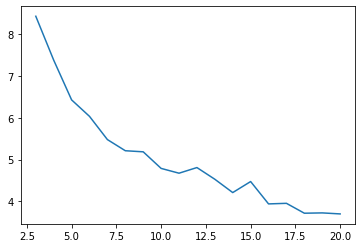
\includegraphics[height=4.5cm,width=7.5cm]{replace.png}
	\caption{不同K值损失函数变化}
	\label{differentK}
\end{figure}

通过上图可以确定全局聚类簇个数为******************

在 MCD-Clustering 算法中的局部聚类过程,K值选取将会影响马尔科夫链对轨迹生成模型的估计,图\ref{differentKJB}展示了局部聚类不同K值下的ARI指数变化。
\begin{figure}[h]
	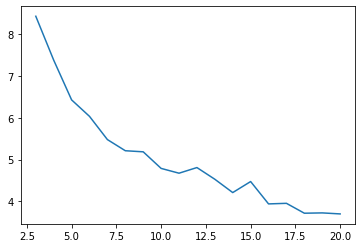
\includegraphics[height=4.5cm,width=7.5cm]{replace.png}
	\caption{局部聚类不同K值对实验结果的影响}
	\label{differentKJB}
\end{figure}

依据上图,可以看到,随着K值增大,ARI指数也会随之增大,即聚类效果更好。这是因为当K值很小时,轨迹子簇中的轨迹相似性不高,可能会有多种走势形状的轨迹存在,通过这样的轨迹子簇数据训练出来的生成模型会生成多种走势形状混合的轨迹数据,而走势性形状混合的轨迹数据在原始轨迹数据中是不存在的,这样就会给后续全局聚类操作造成影响。但随着K值增大,需要在网络中传输更多的转移矩阵,也因此会使网络信息传输压缩率有所降低。

在 MCD-Clustering 算法中对轨迹数据进行了网格化处理,假设网格化粒度记为$\delta$,若$\delta$越大则表示网格化粒度越粗,反之,则网格化粒度越精细。我们对不同网格化粒度情况下 MCD-Clustering 算法的聚类效果进行了实验,实验结果如图\ref{differentDELTA}。
\begin{figure}[h]
	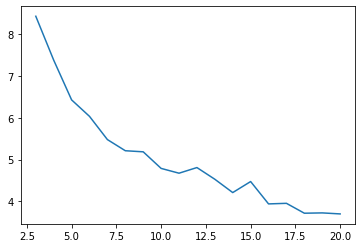
\includegraphics[height=4.5cm,width=7.5cm]{replace.png}
	\caption{不同网格粒度对实验结果的影响}
	\label{differentDELTA}
\end{figure}

从上图可以看出,当网格粒度越来越精细,ARI指数也会随之增大,即聚类效果越来越好。但随着网格粒度越来越精细,需要在网络中传输的转移矩阵会越来越大,也因此会使网络信息传输压缩率有所降低。


\section{本章小结}
